\documentclass{article}
\usepackage[utf8]{inputenc}
\usepackage{graphicx}
\usepackage{wrapfig}
\usepackage{array}
\usepackage{siunitx}
\usepackage{xcolor}
\usepackage{multicol}
\usepackage{amssymb}
\usepackage{hyperref}
\setlength{\columnseprule}{1pt}

\title{Single Phase Transformation B-H Loop \\ Lab Report 8 \\ ELP100}
\author{Yash Agarwal \\ 2021EE10638 \\ Group 29}
\date{June 4, 2022}

\begin{document}
\pagecolor{yellow!15}
\maketitle
\vspace{15px}
\tableofcontents
\newcolumntype{V}{>{\centering\arraybackslash} m{.4\linewidth} }
\newpage
\section{B-H Loop}
\subsection{Aim}
To study the constructional details of a single phase transformer and to display the B-H curve for the core material used, on the oscilloscope for different no load input voltages.

\subsection{Apparatus}
\begin{enumerate}
\item 1 – Phase Transformer of identical ratings
\item 1 – Phase Auto-transformer
\item Low Power-factor Wattmeter
\item AC Ammeter
\item AC Voltmeter

\end{enumerate}

\subsection{Theory}
\begin{center}
    \fcolorbox{black}{white}{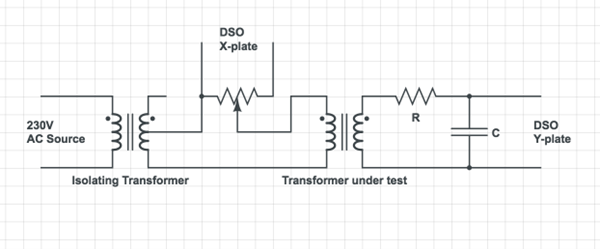
\includegraphics[width=0.9\textwidth]{Picture1.png}}    
\end{center}

When an ac voltage is applied to the primary winding, with the secondary left open circuited the primary current is proportional to the field 'H' and the induced EMF in the secondary winding is proportional to the rate of change of flux (or flux density B). This
is because:
\[ H\propto i\]

If now a signal proportional to the primary current is applied to the horizontal or 'X' plates of the oscilloscope and a signal is applied to the vertical or ‘Y’ plates of oscilloscope, a BH curve is seen on the oscilloscope.

\newpage
\subsection{Observation}
\vspace{5px}
\begin{center}
\vspace{10px}
\begin{tabular}{| V | c | c |} 
 \hline
    \ & \ & \ \\
    Photo & $V_{Input}$ & Resistance\\ [1em]
    \hline
    \ & \ & \ \\
    \fcolorbox{black}{yellow!15}{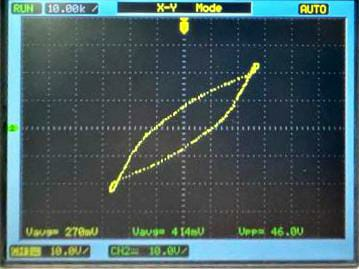
\includegraphics[width=0.35\textwidth]{WhatsApp Image 2022-06-05 at 10.58.46 PM.jpeg}} & 150V & 285.5$\Omega$\\
    \vspace{10px}
    \fcolorbox{black}{yellow!15}{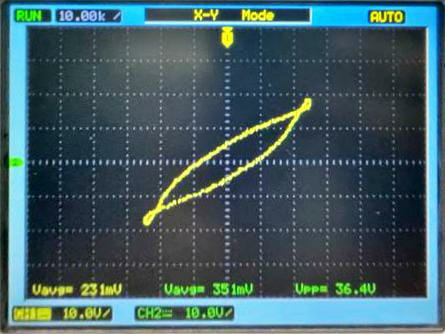
\includegraphics[width=0.35\textwidth]{WhatsApp Image 2022-06-05 at 10.58.45 PM (1).jpeg}} & 120V & 285.5$\Omega$\\
    \vspace{10px}
    \fcolorbox{black}{yellow!15}{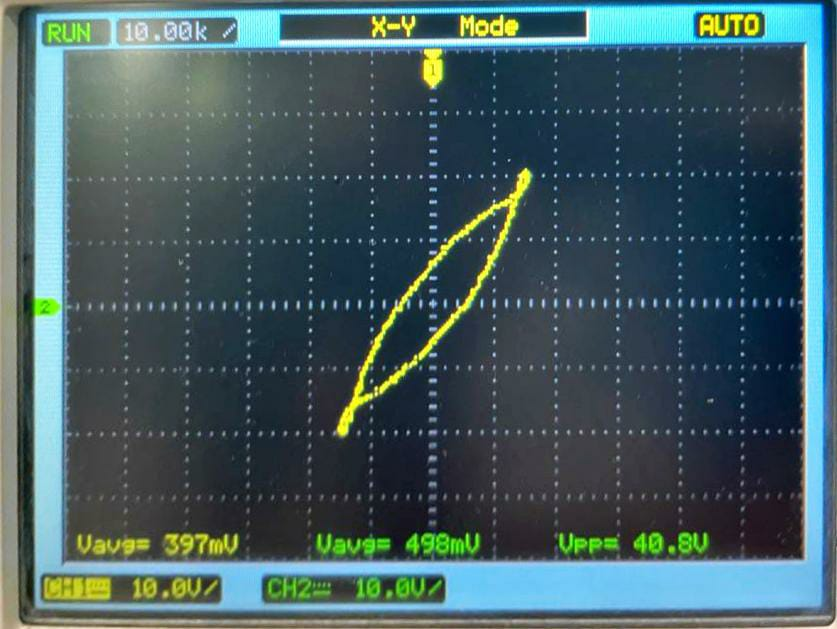
\includegraphics[width=0.35\textwidth]{WhatsApp Image 2022-06-05 at 10.58.44 PM.jpeg}} & 120V & 164.6$\Omega$\\
    \vspace{10px}
    \fcolorbox{black}{yellow!15}{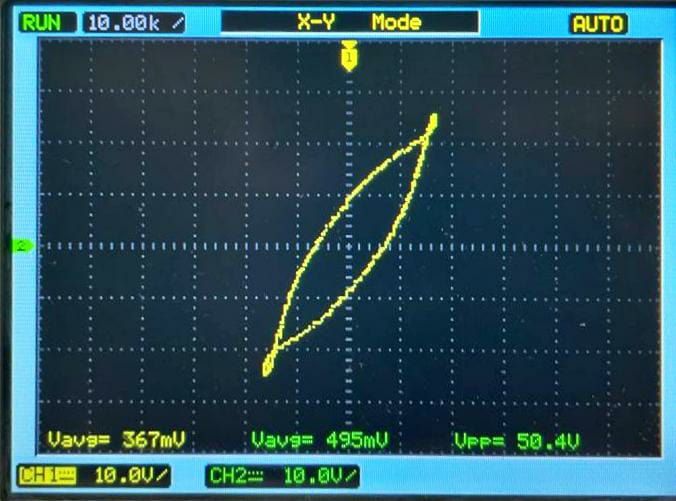
\includegraphics[width=0.35\textwidth]{WhatsApp Image 2022-06-05 at 10.58.45 PM.jpeg}} & 150V & 164.6$\Omega$\\
    \ & \ & \ \\
 \hline
\end{tabular}
\end{center}
\newpage

\subsection{Breadboard Setup}
\vspace{5px}
\begin{center}
\fcolorbox{black}{white}{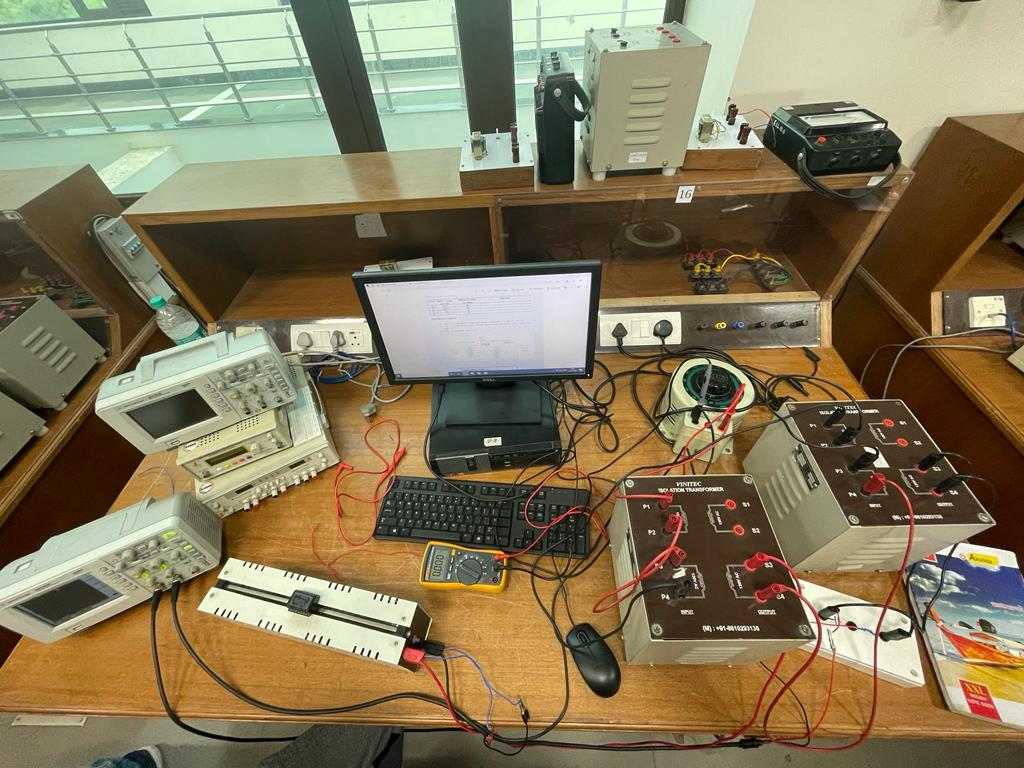
\includegraphics[width=1\columnwidth]{WhatsApp Image 2022-06-05 at 6.13.46 PM (1).jpeg}}
\end{center}
\vspace{20px}

\section{Sources of Error}
\begin{itemize}
\item Scale of DSO not appropriate for measurements
\item Loose Connections
\item Resistance of wires not taken into account, and also giving rise to inconsistency due to increase in resistance due to heating
\item Change in the connections while circuit is closed.

\end{itemize}

\section{Precautions}

\begin{itemize}
\item Make the connections neat and tight
\item Don’t leave the switch on for long continuous periods of time.
\item Wear proper shoes and use insulated tools
\end{itemize}

\section{Concluding Remarks}
On the DSO, the B-H curve for various no load input voltages (thus varying flux densities) can be examined by altering the input supply voltage through autotransformer or by changing the rheostat. We notice the following:
\begin{enumerate}
    \item The B-H Loop behaves as expected in case 1. The Magnetic Field lags the Magnetic Intensity, similar to a generic hysteresis loop.
    \item In Cases 2 and 3, we kept the Autotransformer voltage constant at 120 V but altered the rheostat values to 285.5 and 164.5, respectively, and observed that the voltage across the capacitor varies dramatically but the B-H Loop breadth nearly stays constant.
    \item In Cases 3 and 4, we kept the rheostat resistance constant, = 164.6, but increased the Autotransformer voltage to 150 V. We can see that both B and H values are changing currently.
\end{enumerate}

\end{document}
